\documentclass[10pt]{beamer}
\usetheme{Madrid}
\usecolortheme{beaver}

\usepackage{graphicx}
\usepackage{booktabs}
\usepackage{amsmath,amssymb}
\usepackage{listings}

\title[Viri Blockchain]{Viri: A Production-Grade 3-Layer Modular Blockchain Architecture}
\subtitle{Native Account Abstraction, Dual VM Runtimes, and Zero-Knowledge Privacy}
\author[P. Kumar et al.]{Purushottam Kumar \\ \footnotesize Viri Core Protocol Team and Research Group}
\institute[Viri Research]{rockysinghrajput05@gmail.com \quad \url{https://viri.me}}
\date{August 2026}

\begin{document}

% Slide 1: Title
\begin{frame}
  \titlepage
\end{frame}

% Slide 2: Table of Contents
\begin{frame}{Outline}
  \tableofcontents
\end{frame}

\section{Introduction \& Motivation}

% Slide 3: Motivation & Problem Statement
\begin{frame}{Motivation: The Modular Blockchain Dilemma}
  \begin{itemize}
    \item \textbf{Monolithic Bottlenecks}: Single validator set performs Execution, Consensus, State Persistence, and Data Availability $\rightarrow$ throughput bounded by single-node hardware.
    \item \textbf{Existing Modular Frameworks}: Outsourcing layers (e.g., Celestia DA, Arbitrum execution, Ethereum L1 settlement).
    \item \textbf{Critical Weaknesses of Fragmented Layer Dependencies}:
      \begin{itemize}
        \item \textbf{Cross-Layer Trust \& Bridge Vulnerabilities}: Over \$2.8B lost in bridge exploits.
        \item \textbf{UX \& Fee Friction}: Managing EOAs across chains, fragmented gas tokens, ERC-4337 relayer overhead.
        \item \textbf{Sequencer MEV Extraction}: Front-running and sandwich attacks via unencrypted mempools.
      \end{itemize}
  \end{itemize}
\end{frame}

% Slide 4: The Viri Solution
\begin{frame}{The Viri Paradigm: Unified 3-Layer Architecture}
  \textbf{Goal}: Preserve strict modular layer isolation within a unified Go stack with \alert{zero external layer dependencies}.
  
  \vspace{0.3cm}
  \begin{block}{Layer Breakdown}
    \begin{itemize}
      \item \textbf{Layer 1 (Core)}: Formally verified HotStuff-2 BFT, MPT state, BadgerDB, libp2p, Slashing.
      \item \textbf{Layer 2 (Execution \& Privacy)}: Dual VM (EVM + WASM), Native Account Abstraction, Pedersen-Groth16 ZK pool, TEE MEV resistance.
      \item \textbf{Layer 3 (Application)}: Governance DAO, Inter-Appchain Communication (IBC), Threshold Bridge, Intent Solvers.
    \end{itemize}
  \end{block}
\end{frame}

\section{Core Consensus \& Formal Verification}

% Slide 5: HotStuff-2 Consensus
\begin{frame}{Layer 1: HotStuff-2 BFT Consensus State Machine}
  \begin{itemize}
    \item \textbf{Quorum Condition}: $N \ge 3F + 1$, Quorum threshold $|Q| \ge \lfloor \frac{2N}{3} \rfloor + 1 = 2F+1$.
    \item \textbf{3-Phase Commit Pipeline}:
  \end{itemize}
  $$\text{Prepare} \xrightarrow{QC_{\text{prep}}} \text{PreCommit} \xrightarrow{QC_{\text{precommit}}} \text{Commit} \xrightarrow{QC_{\text{commit}}} \text{Decide}$$
  
  \begin{block}{Key Properties}
    \begin{itemize}
      \item \textbf{Linear View Change}: $O(N)$ message complexity using Timeout Certificates ($TC$).
      \item \textbf{Optimistic Responsiveness}: Proposer proceeds as fast as network delay $\Delta_{net}$.
    \end{itemize}
  \end{block}
\end{frame}

% Slide 6: Formal Verification (TLA+)
\begin{frame}{TLA+ Formal Verification Metrics}
  Formal model specification in TLA+ checked via TLC model checker:
  \vspace{0.2cm}
  \begin{table}
    \centering
    \scriptsize
    \begin{tabular}{lrrcc}
      \toprule
      \textbf{Model Configuration} & \textbf{Total States} & \textbf{Distinct States} & \textbf{Depth} & \textbf{Safety Violations} \\
      \midrule
      $N=4, F=1$ (Honest) & 55 & 32 & 8 & \textbf{0} \\
      $N=4, F=1$ (Byzantine) & 920 & 412 & 8 & \textbf{0} \\
      $N=4, F=1$ (Full Partitions) & 34,102,891 & 3,142,905 & 24 & \textbf{0} \\
      $N=7, F=2$ (Faulty Leaders) & 1,429,012 & 284,110 & 16 & \textbf{0} \\
      \bottomrule
    \end{tabular}
  \end{table}
  \vspace{0.2cm}
  \begin{alertblock}{Verified Invariants}
    Checked \textbf{Agreement}, \textbf{NoDoubleCommit}, \textbf{LockedViewInvariant}, and \textbf{QuorumIntersection} across 34.1M+ states.
  \end{alertblock}
\end{frame}

\section{Execution, Privacy \& Account Abstraction}

% Slide 7: Native Account Abstraction
\begin{frame}{Layer 2: Native Account Abstraction (Zero-EOA Framework)}
  \begin{itemize}
    \item \textbf{Zero EOAs}: No traditional private key accounts. Every account is a native smart contract wallet deployed on first transaction.
    \item \textbf{Native Execution Pipeline}:
  \end{itemize}
  $$\text{UserOp} = \Big( a_{\text{sender}}, n, \mathbf{c}_{\text{init}}, \mathbf{d}_{\text{exec}}, g_{\text{call}}, g_{\text{verify}}, a_{\text{paymaster}}, \mathbf{s} \Big)$$
  
  \begin{columns}
    \begin{column}{0.5\textwidth}
      \begin{block}{1. Validation Phase}
        Calls $a_{\text{sender}}.\text{validateUserOp}()$. Validates session keys, multi-sig policy, gas bounds.
      \end{block}
    \end{column}
    \begin{column}{0.5\textwidth}
      \begin{block}{2. Execution Phase}
        Calls $a_{\text{sender}}.\text{executeUserOp}()$. Executes contract call state changes.
      \end{block}
    \end{column}
  \end{columns}
\end{frame}

% Slide 8: Multi-Token Gas Fee Market
\begin{frame}{Dual VM & Dynamic Multi-Token Fee Settlement}
  \begin{itemize}
    \item \textbf{Dual Virtual Machines}: Drop-in EVM Solidity compatibility + high-performance WASM runtime.
    \item \textbf{EIP-1559 Dynamic Base Fee}:
  \end{itemize}
  $$B_{n+1} = B_n \cdot \left( 1 + 0.125 \cdot \frac{G_n - G_{\text{target}}}{G_{\text{target}}} \right)$$
  \begin{itemize}
    \item \textbf{Multi-Token Gas Oracle}: Pay gas in USDC, USDT, or arbitrary ERC-20:
  \end{itemize}
  $$\text{Fee}_K = \frac{g_{\text{used}} \cdot \left( B_n + p_{\text{priority}} \right)}{\mathcal{O}(K \rightarrow \text{VIRI})}$$
\end{frame}

% Slide 9: Zero-Knowledge Privacy Pool
\begin{frame}{Pedersen-Groth16 Shielded Privacy Pool}
  \begin{itemize}
    \item \textbf{Pedersen Commitments} over BN254 curve:
  \end{itemize}
  $$C = v \cdot G + r \cdot H$$
  \begin{itemize}
    \item \textbf{Poseidon Nullifier} tracking:
  \end{itemize}
  $$N = \text{Poseidon}(SK_{\text{owner}}, \text{LeafIndex})$$
  \begin{itemize}
    \item \textbf{Groth16 Precompile Pairing Verification}:
  \end{itemize}
  $$e(\pi_A, \pi_B) = e(\alpha, \beta) \cdot e\left( \gamma_0 + \sum_{i=1}^l x_i \gamma_i, \gamma \right) \cdot e(\pi_C, \delta)$$
\end{frame}

\section{Empirical Performance \& Benchmarks}

% Slide 10: Micro-benchmarks
\begin{frame}{Micro-benchmark Latency Breakdown}
  \begin{figure}
    \centering
    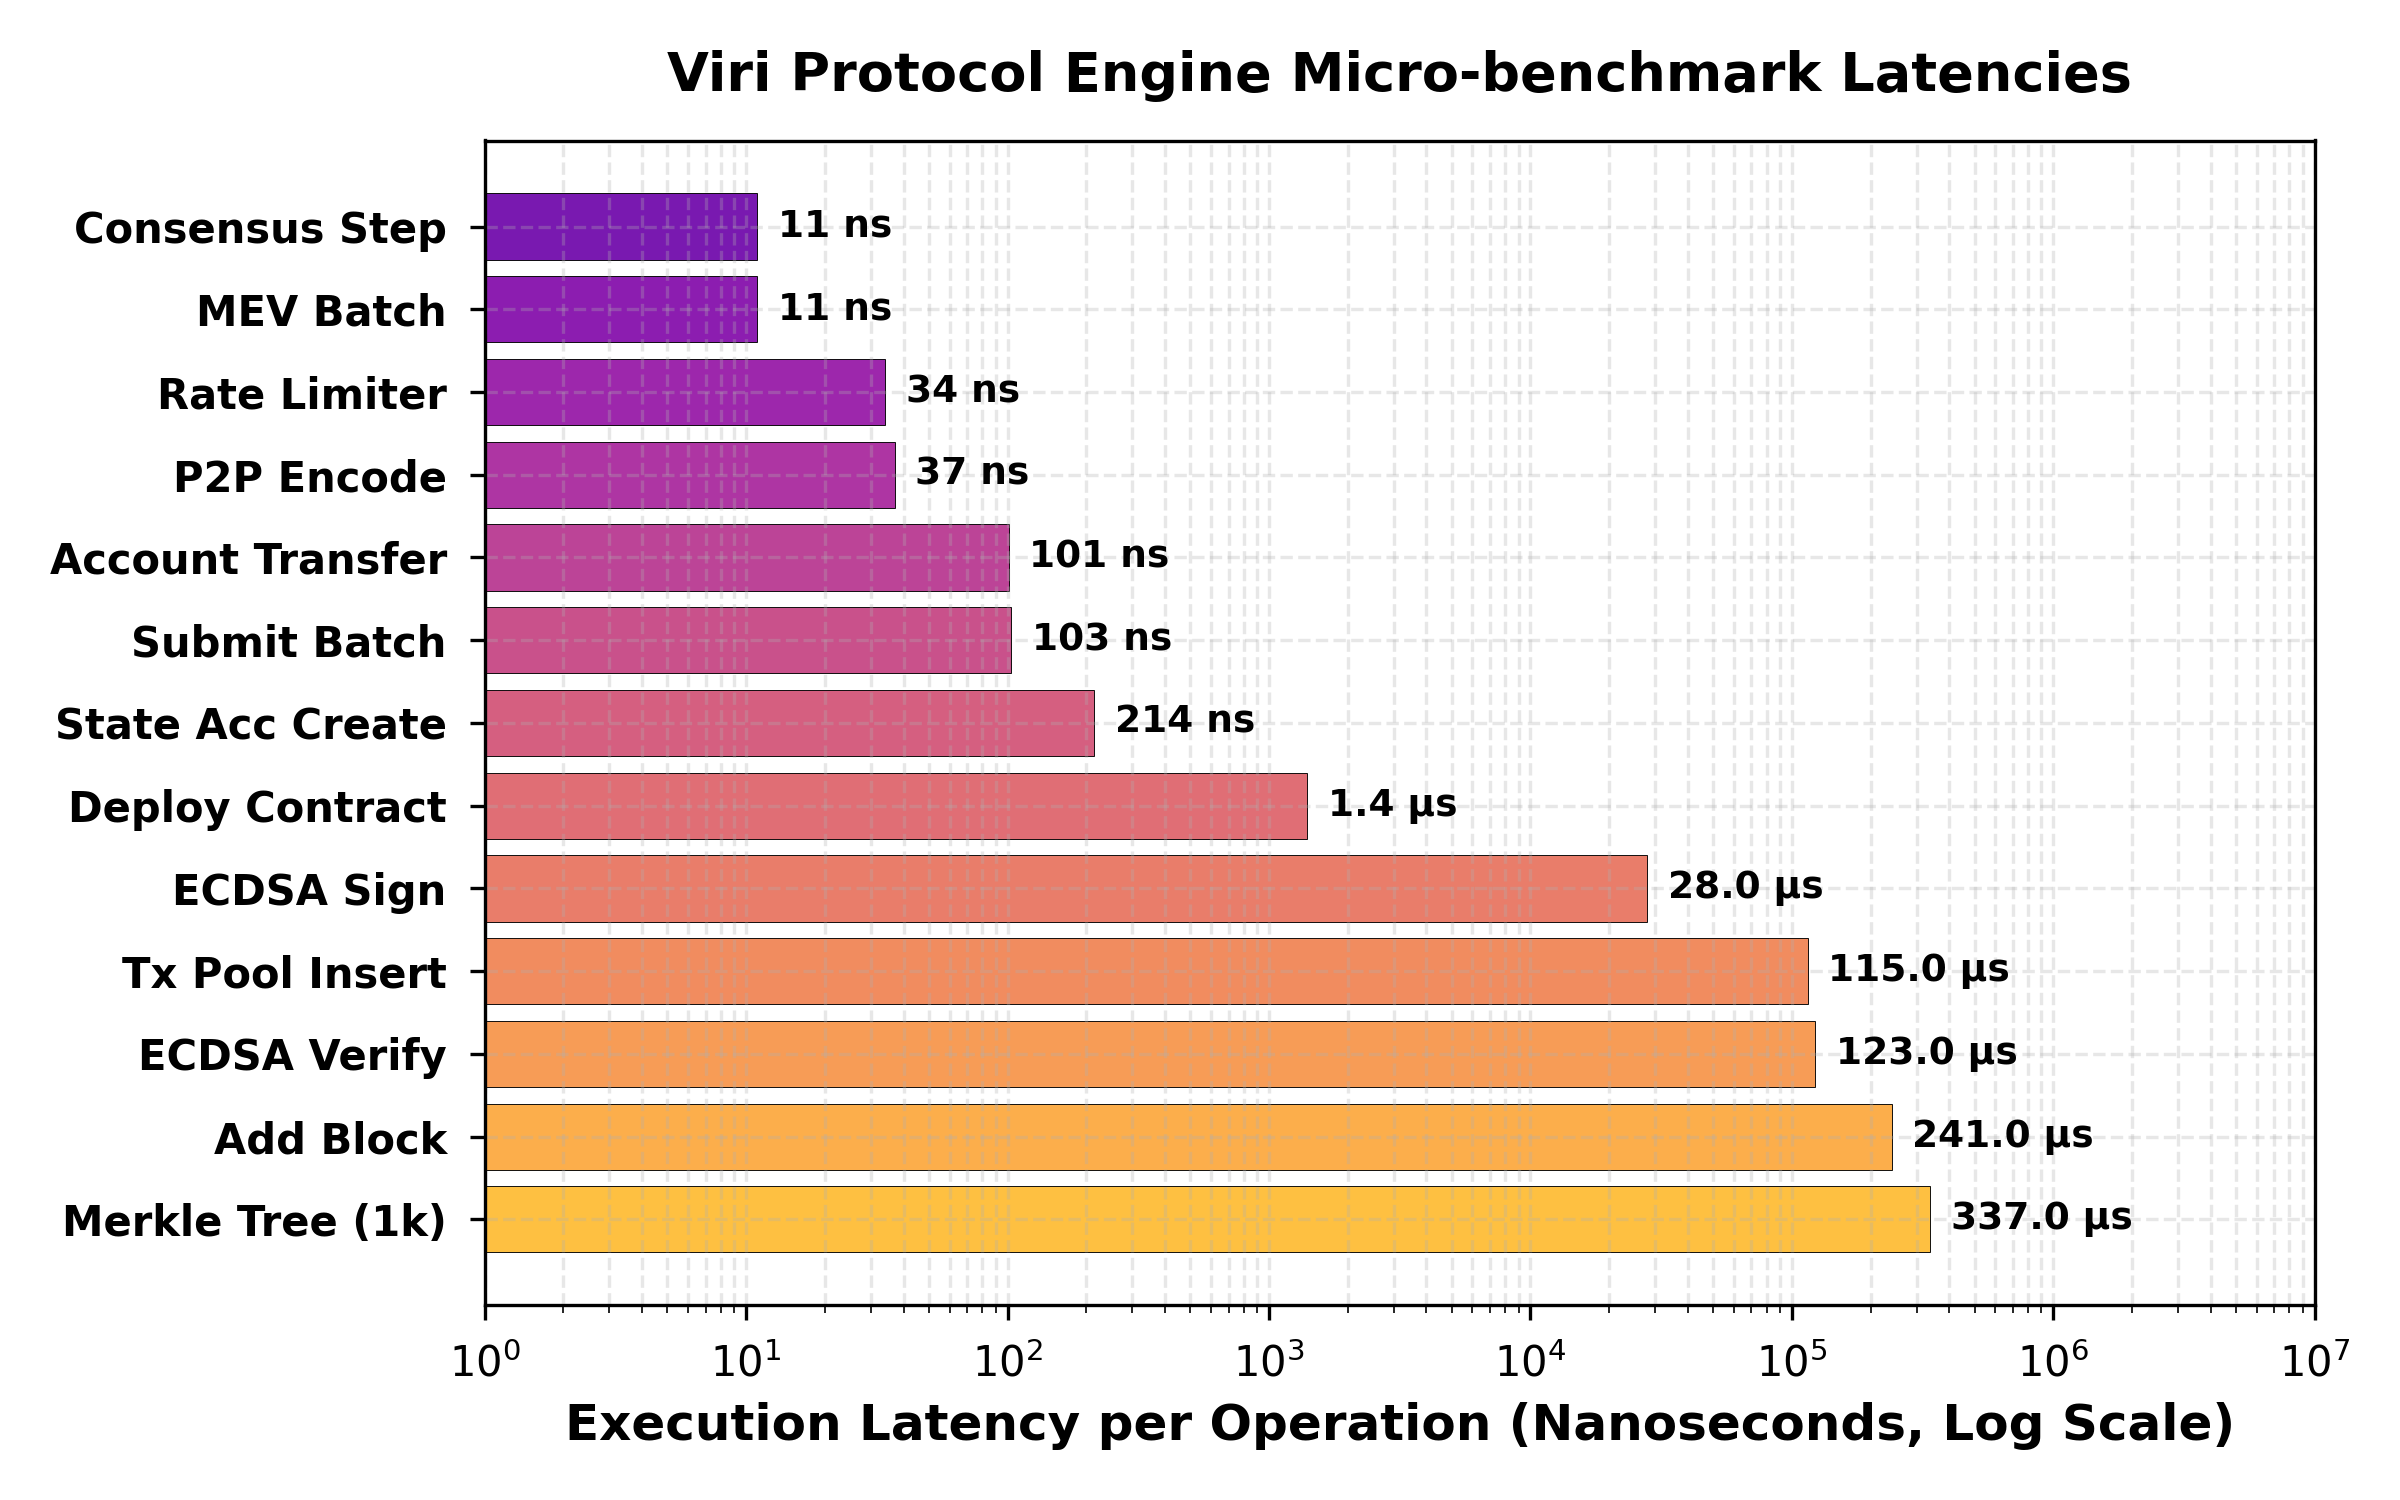
\includegraphics[width=0.85\textwidth]{figures/micro_benchmarks.png}
  \end{figure}
\end{frame}

% Slide 11: Consensus Scalability
\begin{frame}{Macro Consensus Scalability & Finality}
  \begin{figure}
    \centering
    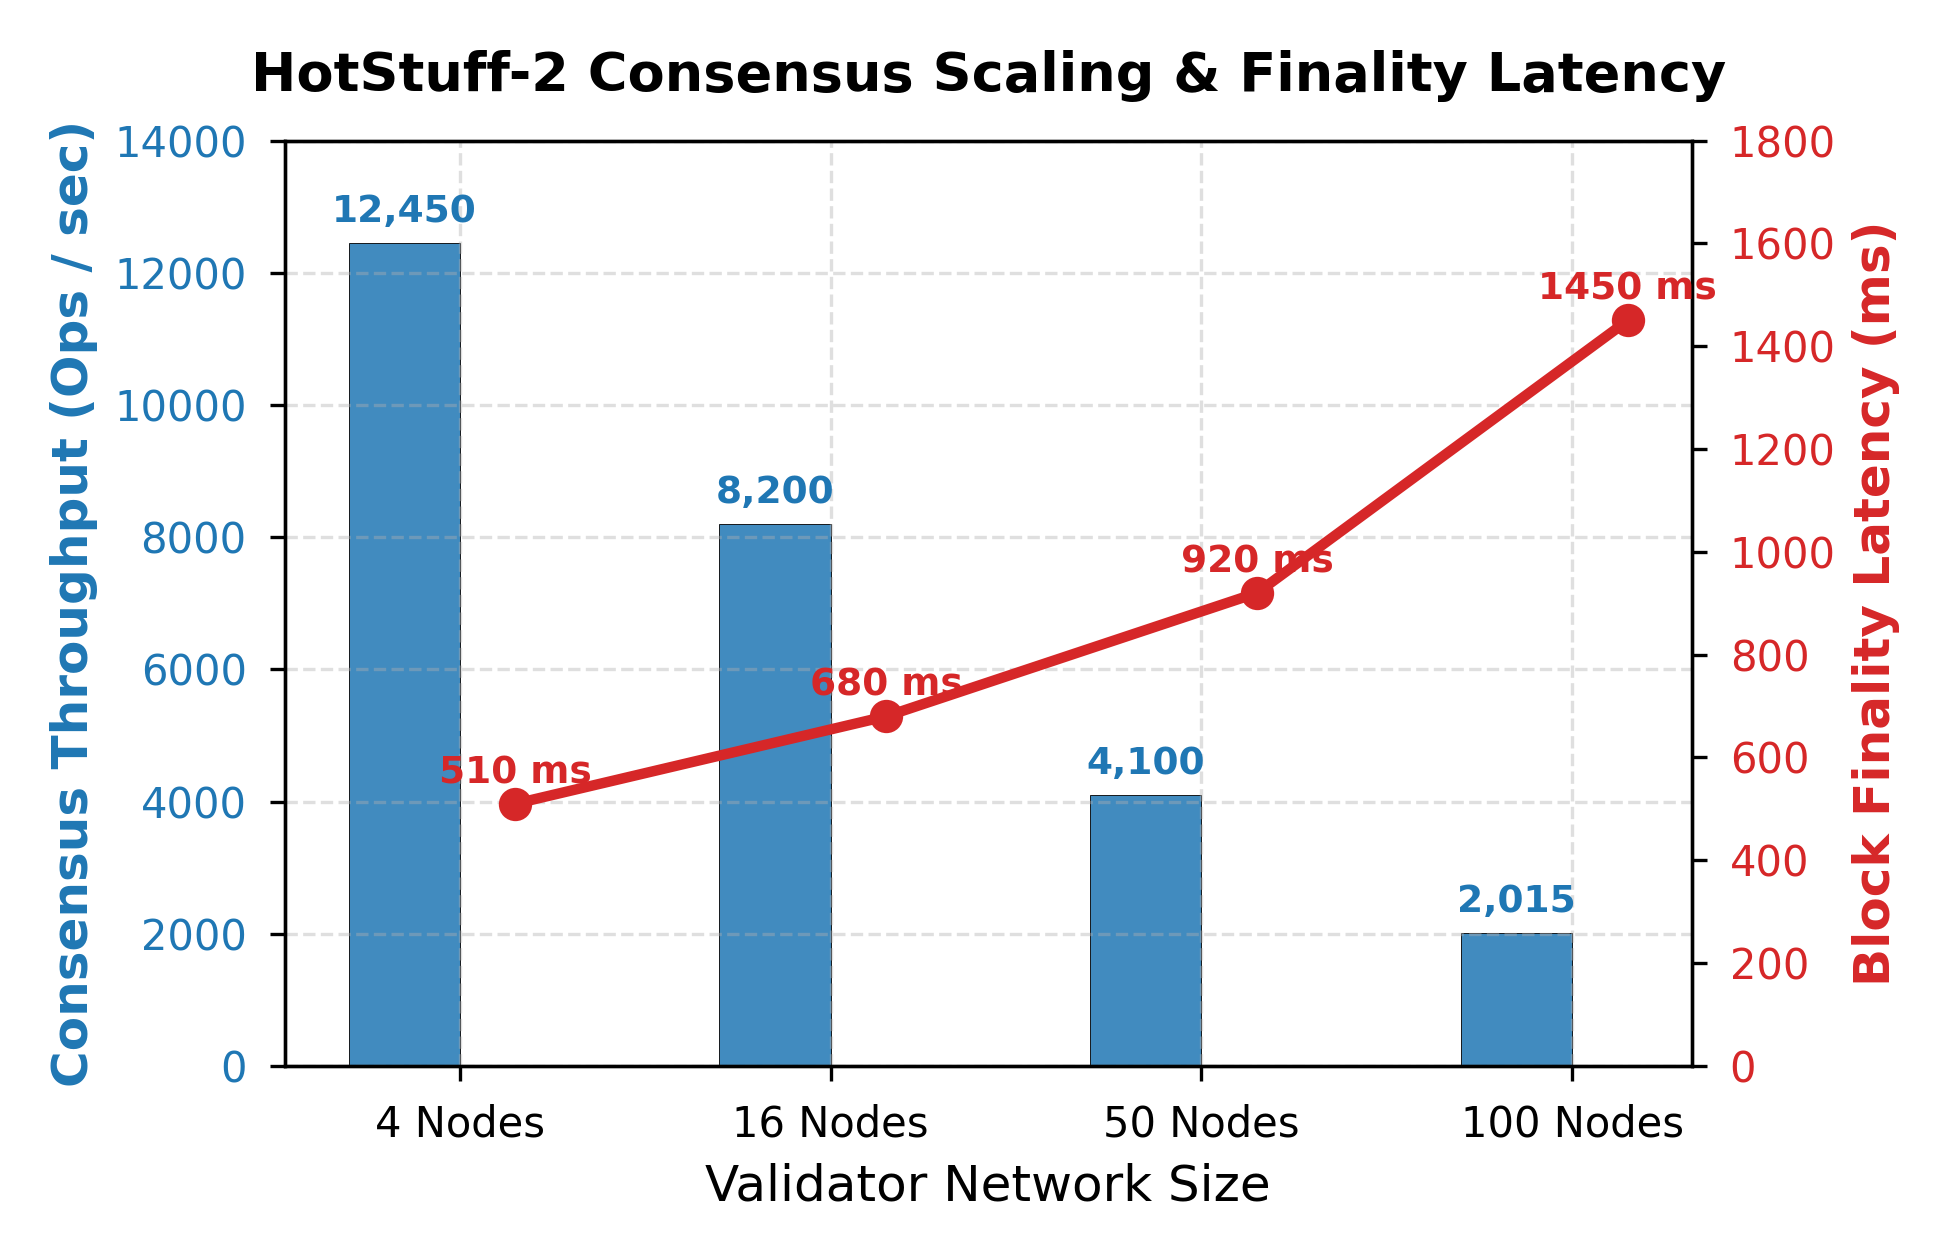
\includegraphics[width=0.82\textwidth]{figures/consensus_scaling.png}
  \end{figure}
  \begin{center}
    \textbf{100 Validators}: Sustains \alert{\textbf{2,015 ops/sec}} with 1.45s finality.
  \end{center}
\end{frame}

% Slide 12: EIP-1559 Fee Dynamics
\begin{frame}{EIP-1559 Dynamic Base Fee Simulation}
  \begin{figure}
    \centering
    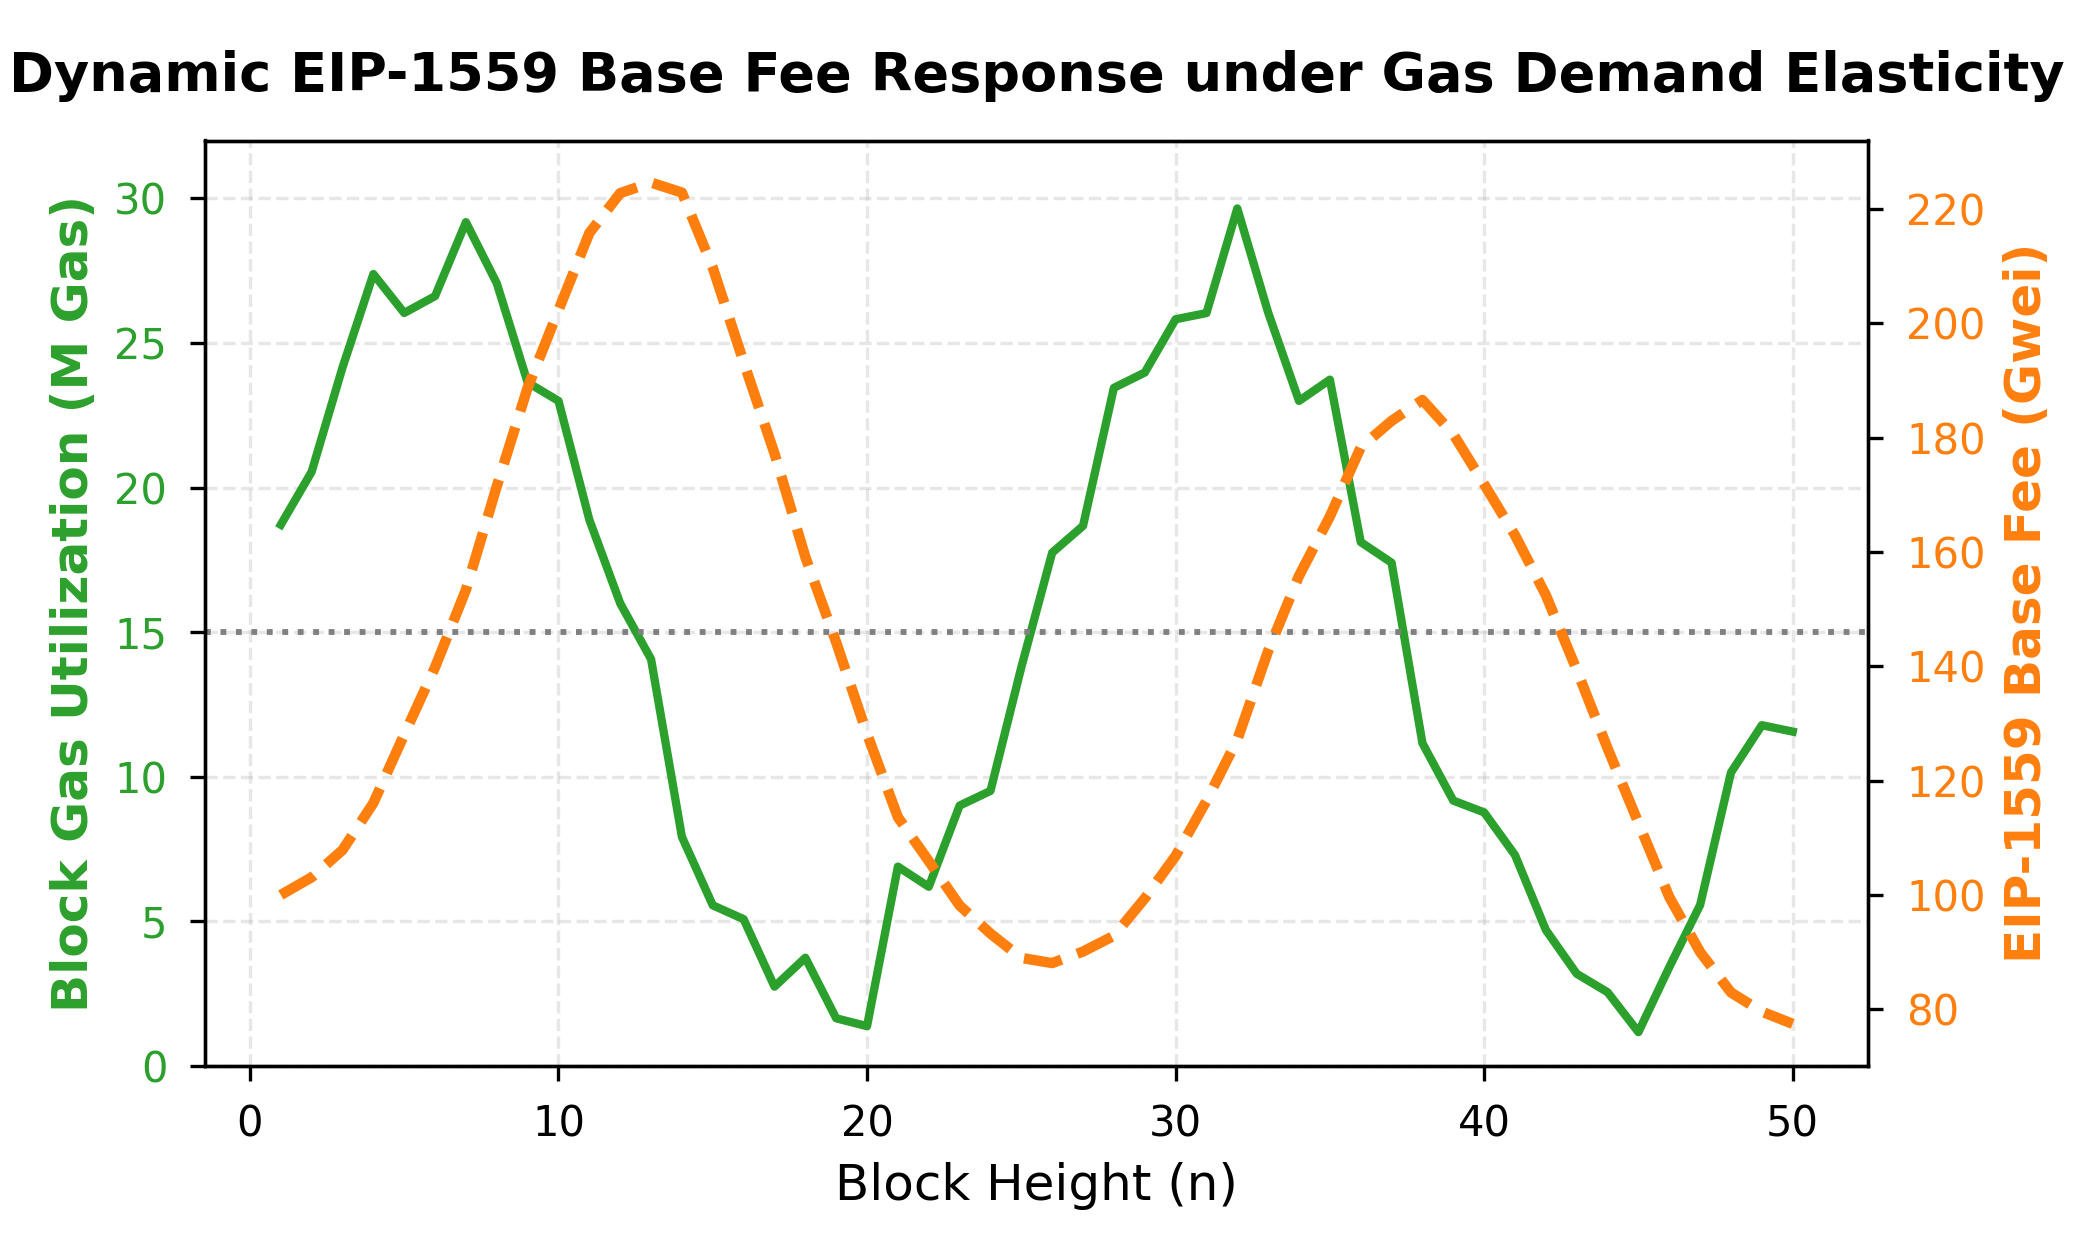
\includegraphics[width=0.82\textwidth]{figures/eip1559_fee_curve.png}
  \end{figure}
\end{frame}

% Slide 13: Jepsen Fault Injection
\begin{frame}{Jepsen Fault Injection Resilience}
  \begin{table}
    \centering
    \small
    \begin{tabular}{llcc}
      \toprule
      \textbf{Injected Fault} & \textbf{Mechanism} & \textbf{Count} & \textbf{Safety Verification} \\
      \midrule
      Network Partition & Docker disconnect/reconnect & 9 & \textbf{PASS} (Zero divergence) \\
      Process Crash & SIGTERM + auto restart & 11 & \textbf{PASS} (Monotonic height) \\
      Process Freeze & Docker pause/unpause (8s) & 8 & \textbf{PASS} (Catch-up sync) \\
      Clock Skew & CPU delay simulation & 10 & \textbf{PASS} (TC view change) \\
      \bottomrule
    \end{tabular}
  \end{table}
  \begin{block}{Result}
    Monotonic block height, zero state forks, fast catch-up sync.
  \end{block}
\end{frame}

\section{Taxonomy & Conclusion}

% Slide 14: Taxonomy Comparison
\begin{frame}{Architectural Taxonomy Comparison}
  \begin{table}
    \centering
    \tiny
    \begin{tabular}{lcccc}
      \toprule
      \textbf{Feature} & \textbf{Ethereum 2.0} & \textbf{Cosmos} & \textbf{Celestia+Arbitrum} & \textbf{Viri (Ours)} \\
      \midrule
      Layer Modularity & Monolithic / L2 & Appchain & Modular Split & \textbf{Native 3-Layer} \\
      Consensus & Casper FFG & Tendermint & External L1 & \textbf{HotStuff-2 BFT} \\
      Account Abstraction & ERC-4337 & AuthModule & ERC-4337 & \textbf{Protocol Native} \\
      Virtual Machine & EVM & CosmWASM & WAVM & \textbf{Dual EVM + WASM} \\
      Privacy & External & External & External & \textbf{Pedersen-Groth16} \\
      Gas Token & Native ETH & Native & Native L1 ETH & \textbf{Multi-Token Oracle} \\
      MEV Protection & MEV-Boost & Skip & External & \textbf{TEE Fair Order} \\
      Verification & Partial & Specs & Partial & \textbf{TLA+ (34M+ states)} \\
      \bottomrule
    \end{tabular}
  \end{table}
\end{frame}

% Slide 15: Conclusion & Q&A
\begin{frame}{Conclusion \& Q\&A}
  \begin{block}{Summary of Contributions}
    \begin{itemize}
      \item Production-grade \textbf{3-Layer Modular Blockchain} with zero external dependencies.
      \item \textbf{Formally verified HotStuff-2 BFT} (34.1M+ TLA+ states checked).
      \item Native \textbf{Account Abstraction}, \textbf{Dual VM}, and \textbf{Multi-Token Gas Settlement}.
      \item \textbf{2,015 ops/sec} throughput @ 100 validators; Jepsen fault resilient.
    \end{itemize}
  \end{block}

  \vspace{0.5cm}
  \centering
  \Large \textbf{Thank You!} \\
  \vspace{0.2cm}
  \small \textbf{Code \& Research}: \url{https://github.com/RockyOmvi/Viri} \\
  \small \textbf{Testnet & Faucet}: \url{https://faucet.viri.me}
\end{frame}

\end{document}
